% This example is meant to be compiled with lualatex
\PassOptionsToPackage{unicode}{hyperref}
\documentclass[aspectratio=1610, 9pt]{beamer}


\usetheme[
  % ShowTotalFrames,               % show total number of frames in the footline
  % ProgressBar,                     % show progressbar
  % ProgressBarStart=1,            % start progressbar at page 1
]{code}


\usepackage{fontspec}
\usepackage[english]{babel}

\usepackage{fontawesome5}

\usepackage{amsmath}
\usepackage{mathtools}
\usepackage{amssymb}
\usepackage{mleftright}

\usepackage[
  math-style=ISO,
  bold-style=ISO,
  sans-style=italic,
  nabla=upright,
  partial=upright,
  mathrm=sym,
]{unicode-math}
\setmathfont{Fira Math}[Scale=MatchLowercase]

\usepackage[
  locale=UK,
  separate-uncertainty=true,
  per-mode=symbol-or-fraction,
]{siunitx}

\usepackage[
  german=quotes,
  autostyle,
]{csquotes}
\usepackage{xfrac}

\usepackage{tabularray}
\UseTblrLibrary{booktabs, siunitx, varwidth}
\usepackage{threeparttable}

\usepackage{graphicx}

\usepackage[
  compatibility=false,
]{caption}
\usepackage{subcaption}

\usepackage{xcolor}
\usepackage{metalogo}
\usepackage{pdflscape}

\usepackage{fancyvrb}
\usepackage[outputdir=build]{minted2}
\setminted{
  autogobble,
  breaklines,
  stripnl=true,
}
\usemintedstyle{code}

\usepackage[
  theorems,
  many,
]{tcolorbox}

\usepackage{adjustbox}

\usepackage{tikz}
\usetikzlibrary{
  arrows,
  arrows.meta,
  graphs,
  graphdrawing,
  positioning,
  shadows,
  shapes,
}

\usepackage[edges]{forest}

\usepackage[
  shortcuts,
]{extdash}

\usepackage[noframe]{showframe}
\usepackage{bookmark}


\tikzset{
    position label/.style={
       below = 3pt,
       text height = 1.5ex,
       text depth = 1ex
    },
    brace/.style={
     decoration={brace},
     decorate
   }
}

\forestset{
  textfile/.style = {
    execute at begin node=\textcolor{cblack}{\faFile*}\space
  },
  batchfile/.style = {
    execute at begin node=\textcolor{cblack}{\faTerminal}\space
  },
  makefile/.style = {
    execute at begin node=\textcolor{cblack}{\faFile}\space
  },
  pythonfile/.style = {
    execute at begin node=\textcolor{cblack}{\faPython}\space
  },
  opened/.style = {execute at begin node=\textcolor{dircolor}{\faFolderOpen}\space},
  closed/.style = {execute at begin node=\textcolor{dircolor}{\faFolder}\space},
  dir tree/.style = {
    grow'=0,
    font=\ttfamily,
    folder,
    fit=band,
    s sep=5pt,
    before computing xy={l=20pt},
    edge={rounded corners=2pt},
  },
  visible on/.style={
    % for tree={
    /tikz/visible on={#1},
    for children={
      edge={/tikz/visible on={#1}}}
    },
}


% This adds a circle with a picture of your choice in it.
% Usage:
% \roundpic[<optional arguments>, e.g. xshift or yshift]\
% {<radius of the cirlce [cm]>}{<picture width [cm]>}{<path_to_picture>}{x pos}{y pos}{label}
% TO BE PUT INSIDE TIKZ ENVIRONMENT (i.e. \begin{tikzpicture} \roundpic... \end{tikzpicture})
\NewDocumentCommand \roundpic {o o m m m m m o}{%
  \node [%
    circle, draw, minimum size=#3, #1,
    path picture = {%
      \node [#2] at (path picture bounding box.center) {%
        \IfNoValueF{#8}{\hyperlink{#8}\begingroup}
        \includegraphics[#4]{#5}
        \IfNoValueF{#8}{\endgroup}
      };
    }
  ] at (#6, #7) {};
}%

\NewDocumentCommand\sectionslide{m o}{%
  {
  \setbeamertemplate{background} {
    \begin{tikzpicture}[remember picture,overlay]
      \node [anchor=north, yshift=0.25cm] at (current page.north) {
        \reflectbox{\includegraphics[height=\pageheight+0.5cm]{images/sec_img.jpg}}
      };
      \fill[black, path fading=titlefade, fading transform={xscale=.3, xshift=-1.25cm}]
          (current page.north west) ++(0cm,1cm) rectangle (current page.south east);
    \end{tikzpicture}
  }
  \begin{frame}
    \begin{tikzpicture}[remember picture,overlay]
      \node [anchor=east, opacity=0.3] at ([xshift=-15pt]current page.east) {#2};
      \node [font=\bfseries\huge] (title) at (current page.center) {#1};
      \draw [tugreen, line width=1.2pt] (title.south west) -- (title.north west);
    \end{tikzpicture}
  \end{frame}
  }
}

% icon href
\NewDocumentCommand \iref { s m m } {%
  \IfBooleanTF{#1}{
    \href{#2}{{\footnotesize{\faExternalLink*}}\,#3}
  }{
    \href{#2}{{\footnotesize{\faExternalLink*}}\,\texttt{#3}}
  }
}

\NewDocumentCommand \cpp {} {%
  C\nolinebreak\hspace{-.05em}\raisebox{.1ex}{\texttt{+}}\nolinebreak\hspace{-.10em}\raisebox{.1ex}{\texttt{+}}
}

\NewDocumentCommand \src { m O{cblack!50!cwhite} } {
  {\tiny\textcolor{#2}{[#1]}}
}



\xdefinecolor{dircolor}{HTML}{f0c481}


\ExplSyntaxOn

\RenewDocumentEnvironment {block} {m o} {
  \IfValueTF{#2}{
    \begin{tcolorbox}[
      adjusted~title=#1,
      #2,
    ]
  }{
    \begin{tcolorbox}[
      adjusted~title=#1,
    ]
  }
}{
  \end{tcolorbox}
}

\RenewDocumentEnvironment {alertblock} {m o} {
  \IfValueTF{#2}{
    \begin{tcolorbox}[
      adjusted~title=#1,
      colframe=alertred,
      #2,
    ]
  }{
    \begin{tcolorbox}[
      adjusted~title=#1,
      colframe=alertred,
    ]
  }
}{
  \end{tcolorbox}
}

\RenewDocumentEnvironment {exampleblock} {m o} {
  \IfValueTF{#2}{
    \begin{tcolorbox}[
      adjusted~title=#1,
      colframe=blue!80!black,
      #2,
    ]
  }{
    \begin{tcolorbox}[
      adjusted~title=#1,
      colframe=blue!80!black,
    ]
  }
}{
  \end{tcolorbox}
}
\ExplSyntaxOff


\tikzset{
  invisible/.style={opacity=0,text opacity=0},
  visible on/.style={alt={#1{}{invisible}}},
  alt/.code args={<#1>#2#3}{%
    \alt<#1>{\pgfkeysalso{#2}}{\pgfkeysalso{#3}} % \pgfkeysalso doesn't change the path
  },
}

\NewDocumentCommand \rtd {} {\textbf{Read}\emph{the}\textbf{Docs}}



% Put settings here, like
\unimathsetup{
  math-style=ISO,
  bold-style=ISO,
  nabla=upright,
  partial=upright,
  mathrm=sym,
}

\NewDocumentCommand \eg {} {e.\,g.}
\NewDocumentCommand \ie {} {i.\,e.}

\title{Python Packaging}
\subtitle{A Brief Recap of the PYOPP Workshop}

\author[A.~Knierim]{Anno Knierim}
\contact{{\large{\faGithub}}\:aknierim}
\date{July 25, 2025}


\begin{document}

\maketitle

\begin{frame}{Why Even Bother With Packaging?}
  \begin{center}
    \huge\textcolor{ccyan!90!cblack}{\textbf{Packages allow you to share your code, so other people can use it.}}
  \end{center}
  \vspace{2em}
  \textcolor{cpink}{But also\dots}
  \begin{itemize}
    \setlength{\itemsep}{1em}
    \item Helps you keeping your code from breaking
    \item Benefits other people that may have faced a similar problem
    \item Saves time because code can be reused easily
  \end{itemize}
\end{frame}

\begin{frame}{Before We Start: Package and Environment Managers}
  \begin{description}
    \setlength{\itemsep}{1em}
    \item [\iref{https://pypi.org/project/pip/}{pip}] The standard package installer for Python. \texttt{pip} is able to install
      directly from PyPI and other indexes.
    \item [\iref{https://mamba.readthedocs.io/en/latest/}{mamba}] Fast and robust, with cross-platform support. Written in \cpp.
      Allows you to manage multiple, isolated environments. \texttt{mamba} installs from local or remote package repositories, \eg, channels.
    \item [\iref{https://python-poetry.org/}{poetry}] Package installer that is also able to create its own virtual environments.
      Handles dependency resolving better than pip. Works nicely with \texttt{pyproject.toml} files. Allows the use of lock files.
    \item [\iref{https://docs.astral.sh/uv/}{uv}] A new and fast package manager written in {\footnotesize{\faRust}}\,\texttt{Rust}. Can create
      virtual environments, and solves dependencies better and faster than pip. Allows the use of lock files.
  \end{description}
  \begin{center}
    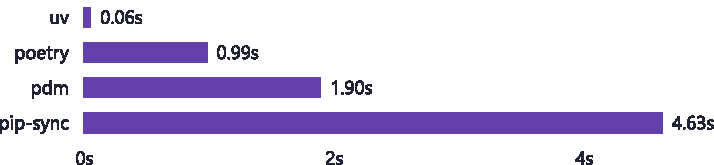
\includegraphics[width=0.7\textwidth]{graphics/speed.pdf}
    \src{docs.astral.sh/uv}
  \end{center}
\end{frame}





\secslide[\fontsize{1.3cm}{1.3cm}\selectfont]{Packaging: The Basics}


\begin{frame}{What Even is a Package?}
  \begin{description}[\texttt{Distribution Package}]
    \setlength{\itemsep}{1.5em}
    \item [\texttt{Import Package}] Any Python module that you can \emph{import} using the \mintinline{python}+import+
      statement.
    \item [\texttt{Namespace Package}] Packages that allow you to \emph{unify} two packages with the \emph{same} name.
    \item [\texttt{Distribution Package}] An archive containing a \emph{collection} of import packages combined with
      \emph{metadata} such as dependencies.
  \end{description}
  \vspace{1cm}
  \uncover<2>{
  \begin{center}
    \huge\textcolor{ccyan}{When people talk about packages, they usually mean \textbf{distribution packages.}}
  \end{center}
  }
\end{frame}

\begin{darkframe}{How Does Python Find Installed Packages?}
  \begin{center}
  \huge\textcolor{ccyan}{Example: NumPy}
  \end{center}
  \vspace{0.5cm}
  \begin{minted}{shell-session}
    $ python -c "import numpy; print(numpy.__path__[0])"
    /home/anno/.local/conda/envs/pyopp_recap/lib/python3.12/site-packages/numpy

    $ ls -C $(python -c "import numpy; print(numpy.__path__[0])") | sort
    _array_api_info.py     doc		      __init__.py	 py.typed
    _array_api_info.pyi    dtypes.py	      __init__.pyi	 random
    char		      dtypes.pyi	      lib		 rec
    __config__.py	      exceptions.py	      linalg		 strings
    __config__.pyi	      exceptions.pyi	      ma		 testing
    _configtool.py	      _expired_attrs_2_0.py   matlib.py	 tests
    _configtool.pyi        _expired_attrs_2_0.pyi  matlib.pyi	 _typing
    conftest.py	      f2py		      matrixlib	 typing
    _core		      fft		      polynomial	 _utils
    core		      _globals.py	      __pycache__	 version.py
    ctypeslib	      _globals.pyi	      _pyinstaller	 version.pyi
    _distributor_init.pyi  __init__.pxd	      _pytesttester.pyi
    _distributor_init.py   __init__.cython-30.pxd  _pytesttester.py
  \end{minted}
\end{darkframe}


\begin{frame}[fragile]{How Do I Create a Package?}
  \begin{center}
    \huge\textcolor{ccyan!90!cblack}{\textbf{There is not \enquote{just one way} to create packages, but\dots}}
  \end{center}
  \vspace{1em}
  \begin{itemize}
    \setlength{\itemsep}{1em}
    \item Modern packaging uses a scaffolding called \texttt{pyproject.toml} with three important sections:
    \begin{description}[\texttt{[build-system]}]
      \item [\mintinline{toml}{[build-system]}] Allows you to describe what build backend to use.
      \item [\mintinline{toml}{[project]}] Sets up metadata for the package, such as the name or version.
      \item [\mintinline{toml}{[tool]}] A section for tool configuration.
    \end{description}
    \item An easy way to set up that scaffolding: \href{https://hatch.pypa.io/latest/}{{\footnotesize{\faExternalLink*}}\,\texttt{hatch}}
      \begin{minted}{shell-session}
        $ uv pip install hatch
        $ mamba install hatch
      \end{minted}
  \end{itemize}
\end{frame}

\begin{splitframe}[fragile]{How Do I Create a Package?}{Output}
  \begin{columns}[t,onlytextwidth]
    \begin{column}{0.58\textwidth}
      \begin{itemize}
        \item Use \textcolor{cpink}{\texttt{hatch}}'s CLI tool to quickstart creating a package:
          \begin{minted}{shell-session}
            $ hatch new my_package
          \end{minted}
      \end{itemize}
    \end{column}
    \hfill
    \begin{column}{0.38\textwidth}
      \begin{minted}{toml}
        my_package
        ├── src
        │   └── my_package
        │       ├── __about__.py
        │       └── __init__.py
        ├── tests
        │   └── __init__.py
        ├── LICENSE.txt
        ├── README.md
        └── pyproject.toml
      \end{minted}
    \end{column}
  \end{columns}
  \vspace{1em}
  \begin{columns}[t,onlytextwidth]
    \begin{column}{0.58\textwidth}
      \begin{itemize}
        \setlength{\itemsep}{1em}
        \item Let's see what this created:
          \begin{minted}{shell-session}
            $ head my_package/pyproject.toml
          \end{minted}
        \item You can also upgrade an existing project to use \texttt{hatch}:
          \begin{minted}{shell-session}
            $ hatch new --init
          \end{minted}
        \item Have a look at the \href{https://packaging.python.org/en/latest/guides/writing-pyproject-toml/}{{\footnotesize{\faExternalLink*}}\,Writing your \texttt{pyproject.toml}}
          guide to learn how to customise the \texttt{pyproject.toml} file
      \end{itemize}
    \end{column}
    \begin{column}{0.38\textwidth}
      \begin{minted}{toml}
        [build-system]
        requires = ["hatchling"]
        build-backend = "hatchling.build"

        [project]
        name = "my_package"
        dynamic = ["version"]
        description = ''
        readme = "README.md"
        requires-python = ">=3.8"
      \end{minted}
    \end{column}
  \end{columns}
\end{splitframe}

\begin{splitframe}[fragile]{Dependencies}{Example}
  \begin{columns}[t,onlytextwidth]
    \begin{column}{0.58\textwidth}
      \begin{itemize}
        \setlength{\itemsep}{1em}
        \item Dependencies for your project are defined with the \texttt{dependencies}
          key inside the \texttt{[project]} section
        \item You can set \href{https://packaging.python.org/en/latest/specifications/dependency-specifiers/}{{\footnotesize{\faExternalLink*}}\,dependency specifiers}
          (aka constraints) such as versions
      \end{itemize}
    \end{column}
    \hfill
    \begin{column}{0.38\textwidth}
      \begin{minted}{toml}
        [project]
        dependencies = [
          "numpy",
          "astropy<=6.1.0",
          "tomli;python_version<'3.11'",
        ]
      \end{minted}
    \end{column}
  \end{columns}
  \vspace{1em}
  \begin{columns}[t,onlytextwidth]
    \begin{column}{0.58\textwidth}
      \begin{itemize}
        \setlength{\itemsep}{1em}
        \item Define your optional dependencies in the \texttt{[project.optional-dependencies]} section
          and group them
        \item Install optional dependencies using
          {
          \usemintedstyle{code-light}
          \begin{minted}{shell-session}
            $ uv pip install my_package[plot]
            $ uv pip install "my_package[plot]"
          \end{minted}
          }
      \end{itemize}
    \end{column}
    \hfill
    \begin{column}{0.38\textwidth}
      \begin{minted}{toml}
        [project.optional-dependencies]
        plot = ["matplotlib"]
      \end{minted}
    \end{column}
  \end{columns}
  \vspace{1em}
\end{splitframe}

\begin{splitframe}[fragile]{Dependency Groups}{Example}
  \begin{columns}[t,onlytextwidth]
    \begin{column}{0.58\textwidth}
      \begin{itemize}
        \setlength{\itemsep}{1em}
        \item Fairly new (accepted \texttt{2024-10-10}): \href{https://peps.python.org/pep-0735/}{{\footnotesize{\faExternalLink*}}\,\texttt{PEP 735}} Dependency Groups
        \item Optional dependencies that are \emph{not} installed when a \emph{user} installs the package, \eg, via PyPI
          \begin{itemize}
            \item [\to] Prevent users from installing dev tools
          \end{itemize}
        \item Install the groups from within your source repo:
          \begin{minted}{shell-session}
            $ uv pip install --group dev
          \end{minted}
      \end{itemize}
    \end{column}
    \hfill
    \begin{column}{0.38\textwidth}
      \begin{minted}{toml}
        [dependency-groups]
        tests = ["pytest", "pytest-cov"]
        docs = ["sphinx"]
        dev = [
          "jupyter",
          "pre-commit",
          {include-group = "tests"},
          {include-group = "docs"},
        ]
      \end{minted}
    \end{column}
  \end{columns}
\end{splitframe}

\secslide[\fontsize{1.2cm}{1.2cm}\selectfont]{Packaging: The Fun Stuff}

\begin{splitframe}[fragile]{CLI Scripts}{Example}
  \begin{columns}[t,onlytextwidth]
    \begin{column}{0.58\textwidth}
      \begin{itemize}
        \setlength{\itemsep}{1em}
        \item We can expose scripts in our package using the \texttt{pyproject.toml}
          \texttt{[project.scripts]} section
        \item Similarly: Entry points, that allow the creation of plugins, and cross-platform
          compatibility
          \begin{itemize}
            \item [\textcolor{cpink}{\to}] See \href{https://setuptools.pypa.io/en/latest/userguide/entry_point.html}{{\footnotesize{\faExternalLink*}}\,Entry Points}
          \end{itemize}
      \end{itemize}
    \end{column}
    \hfill
    \begin{column}{0.38\textwidth}
      \begin{minted}{toml}
        src/my_package/cli.py:
      \end{minted}
      \vspace{0.25em}
      \begin{minted}{python}
        def print_message():
            print("Hello World!")
            raise SystemExit(1)
      \end{minted}
      \vspace{1em}
      \begin{minted}{toml}
        pyproject.toml:
      \end{minted}
      \vspace{0.25em}
      \begin{minted}{toml}
        [project.scripts]
        hello-world = "my_package.cli:print_message"
      \end{minted}
      \vspace{1em}
      \begin{center}
        \huge\textcolor{cpink}{\texttt{\textbf{Result}}}
      \end{center}
      \begin{minted}[escapeinside=||]{toml}
        |\textbf{\textcolor{cpink}{\$}}| hello-world
        Hello World!
      \end{minted}
    \end{column}
  \end{columns}
\end{splitframe}


\begin{darkframe}{Versioning}
  Remember:
  \begin{itemize}
    \item \texttt{pyproject.toml} has required fields:
    \begin{minted}{toml}
      [project]
      name = "my_package"
      version = "0.1.0"
    \end{minted}
    \item One way to get this version is with \texttt{hatch}
    \begin{minted}{shell-session}
      $ hatch version
      0.1.0
    \end{minted}
    \item We can also set a new version using \texttt{hatch}:
    \begin{minted}{shell-session}
      $ hatch version 0.2.0
      Old: 0.1.0
      New: 0.2.0
    \end{minted}
  \end{itemize}
\end{darkframe}

\begin{darkframe}{}
  \begin{tikzpicture}[
      remember picture,
      overlay,
      every node/.style={cpink, font=\bfseries\fontsize{2cm}{1cm}\selectfont},
    ]
    \node [align=left] (svs) at (current page.center) {Static\\Versions\\[0.15\baselineskip]Suck
      \hspace{0.1ex}\Large \textcolor{ccyan}{I guess\dots}};
    \node [ccyan, font=\Large, anchor=west] at ([xshift=1.3cm,yshift=-0.9cm]svs.west) {\emph{kinda}};
  \end{tikzpicture}
\end{darkframe}

\begin{splitframe}[fragile]{So Let's Do Something About It}{Code}
  \begin{columns}[t,onlytextwidth]
    {
      \usemintedstyle{code-light}
    \begin{column}{0.58\textwidth}
      \textbf{\textcolor{ccyan}{Approach \#1:}}
      \begin{itemize}
        \item We can set the \texttt{version} field to dynamic\dots
        \item \dots and set the version as \mintinline{python}+__version__ = "0.1.0"+
        in \texttt{\_\_init\_\_.py}
      \end{itemize}
    \end{column}
    }
    \begin{column}{0.38\textwidth}
      \begin{minted}{toml}
        # pyproject.toml
        [project]
        name = "my_package"
        dynamic = ["version"]

        [tool.hatch.version]
        source = "regex"
        path = "src/my_package/__init__.py"
      \end{minted}
      \vspace{1cm}
      \begin{minted}{python}
        # src/my_package/__init__.py
        __version__ = "0.1.0"
      \end{minted}
    \end{column}
  \end{columns}
\end{splitframe}

\begin{splitframe}[fragile]{So Let's Do Something About It}{Code}
  \begin{columns}[t,onlytextwidth]
    {
      \usemintedstyle{code-light}
    \begin{column}{0.58\textwidth}
      \textbf{\textcolor{ccyan}{Approach \#2:}}
      \begin{itemize}
        \setlength{\itemsep}{1em}
        \item We can set the \texttt{version} field to dynamic\dots
        \item \dots and use the version control system (\eg, \texttt{git})
          to determine the version for us
        \item We can then import the version from the file generated by \texttt{hatch-vcs}
      \end{itemize}
    \end{column}
    }
    \begin{column}{0.38\textwidth}
      \small
      \begin{minted}{toml}
        # pyproject.toml
        [build-system]
        requires = ["hatchling", "hatch-vcs"]
        build-backend = "hatchling.build"

        [project]
        name = "my_package"
        dynamic = ["version"]

        [tool.hatch.version]
        source = "vcs"

        [tool.hatch.build.hooks.vcs]
        version-file = "src/my_package/_version.py"
      \end{minted}
      \vspace{1em}
      \begin{minted}{python}
        # src/my_package/__init__.py
        from ._version import version

        __version__ = version
      \end{minted}
    \end{column}
  \end{columns}
\end{splitframe}

\begin{frame}{File Selection}
  \begin{center}
    \Large\textcolor{ccyan}{Hatch respects your \texttt{.gitignore} for what to include in each type
    of distribution:}
  \end{center}
  \begin{description}
    \item [\iref{https://packaging.python.org/en/latest/specifications/source-distribution-format/}{SDist}]
      Hatch will include everything \emph{not} included in \texttt{.gitignore}, unless told otherwise.
    \item [\iref{https://peps.python.org/pep-0427/}{Wheels}] Everything in \texttt{src/<project>/} excluding files in
    your \texttt{.gitignore}.
  \end{description}
\end{frame}

\begin{darkframe}[fragile]{Rewriting Paths}
  \begin{center}
    \Large\textcolor{ccyan}{\texttt{hatchling} can also move files around and rewrite paths in your Distribution package:}
  \end{center}
  \begin{minted}{toml}
    [tool.hatch.build.targets.wheel]
    include = ["src/my_package", "a-folder"]


    [tool.hatch.build.targets.wheel.sources]
    "src/my_package" = "my_package"
    "a-folder" = "my_package/renamed_folder"
  \end{minted}
\end{darkframe}

\begin{frame}{Data Files}
  \begin{description}
    \item [Data Files] Any files intended for use at \emph{runtime} that are shipped with your package
    and are not code.
  \end{description}

  \begin{itemize}
    \setlength{\itemsep}{1em}
    \item [\to] Can be configuration files or examples
    \item [\to] Data files are best put in a well-defined directory that can be accessed by users
  \end{itemize}
\end{frame}

\begin{darkframe}{Data Files}
  \begin{itemize}
    \item Set up your data files in your \texttt{pyproject.toml}:
      \begin{minted}{toml}
        [tool.hatch.build.targets.wheel.shared-data]
        "a-file.json" = "share/a-file.json"
        "a-directory" = "etc/a-directory"
      \end{minted}
    \item Access them, \eg, using \texttt{sysconfig} or \texttt{importlib}
      \begin{minted}{python}
        # with sysconfig
        import sysconfig

        root = sysconfig.get_path("data", sysconfig.get_default_scheme())
        file_path = root + "/share/a-file.json"
      \end{minted}
      \vspace{1.5em}
      
      \begin{minted}{python}
        # with importlib_resources
        from importlib_resources import files

        file_path = files("my_package").joinpath("a-file")
      \end{minted}
  \end{itemize}
\end{darkframe}

\begin{darkframe}{Building and Inspecting a Wheel (Try It)}
  \begin{itemize}
    \setlength{\itemsep}{1.5em}
  \item A local package:
  \begin{minted}{shell-session}
   $ hatch build -t wheel:editable .
   $ zipinfo ./my_package*.whl
  \end{minted}

  \item Or a package from PyPI:
  \begin{minted}{shell-session}
    $ pip wheel --quiet --no-deps pyvisgen
    $ zipinfo ./pyvisgen*.whl
  \end{minted}
  \end{itemize}
\end{darkframe}

\begin{frame}{Further Reading: Packaging}
  \begin{itemize}
    \setlength{\itemsep}{1em}
    \item \iref{https://agoose77.github.io/packaging-pyopp-2025/}{Packaging in Python (Angus Hollands)}
    \item \iref{https://packaging.python.org/en/latest/}{Python Packaging User Guide}
    \item \iref{https://www.pypa.io/en/latest/}{Python Packaging Authority}
    \item \iref{https://hatch.pypa.io/latest/}{hatch}
    \item \iref{https://docs.astral.sh/uv/}{uv}
    \item \iref{https://mamba.readthedocs.io/en/latest/}{mamba}
    \item \iref{https://learn.scientific-python.org/development/}{Scientific Python Library Development Guide}
    \item \iref{https://learn.scientific-python.org/development/patterns/data-files/}{https://learn.scientific-python.org/development/patterns/data-files/}
  \end{itemize}
\end{frame}

\secslide{Code Quality}

\begin{darkframe}
  \begin{center}
    \uncover<2>{
      
\includegraphics[width=0.35\textwidth]{graphics/patrick.jpg}
    }
    \\[1.5em]
    \begin{minipage}{0.8\textwidth}
      \begin{minted}{python}
        def f(x,y=0):return[x[i]+y if x[i]>0else y-x[i]for i in range(len(x))]
      \end{minted}
    \end{minipage}
    \\[3em]
    \uncover<2>{
      \huge\textcolor{ccyan}{This runs, but do you trust it?}
    }
  \end{center}

  \begin{tikzpicture}[remember picture, overlay]
    \coordinate (pos) at ([xshift=-2cm, yshift=1cm]current page.south east);
    \node [rotate around={30:(pos)}, align=center] at (pos) {Shamelessly taken from\\Stefan's talk :)};
  \end{tikzpicture}
\end{darkframe}

\begin{darkframe}{Code Quality Terminology}
  \Huge
  \begin{enumerate}
    \setlength{\itemsep}{2em}
    \item \textcolor{ccyan}{Surface Quality}
      \begin{itemize}
        \item [\to] Formatting: Layout, naming conventions, whitespaces
      \end{itemize}
    \item \textcolor{ccyan}{Semantic Quality}
      \begin{itemize}
        \item [\to] Docstrings, type hinting
      \end{itemize}
    \item \textcolor{ccyan}{Testability}
      \begin{itemize}
        \item [\to] Writing (simple) code that is easy to test
      \end{itemize}
  \end{enumerate}
\end{darkframe}

\begin{frame}{Surface Quality: PEP 8}
  \begin{center}
    \huge\iref{https://peps.python.org/pep-0008/}{Python Enhancement Proposal No. 8 (PEP 8)}
  \end{center}
  \begin{itemize}
    \setlength{\itemsep}{1em}
    \item Coding convention comprising the standard library, all about readability
    \item Key Aspects:\\
      \begin{center}
      \begin{tblr}{
          colspec={c c c},
          rows={font=\bfseries\Large, fg=ccyan, rowsep=0.25cm},
          columns={colsep=0.75cm},
        }
        Code Layout & String Quotes & Whitespaces \\
        Trailing Commas & Comments & Naming Conventions
      \end{tblr}
      \end{center}
  \end{itemize}
\end{frame}

\begin{darkframe}[fragile]{Surface Quality: PEP 8}
  \begin{center}
    \begin{tikzpicture}[remember picture]
      \node [anchor=east, outer sep=10pt] (wrong) at ([xshift=-1cm]current page.center) {
      \begin{minipage}{0.3\textwidth}
        \begin{minted}{python}
          def add(a, b): return a+b
          from rich import print
          import os, math
          def printPi():print(math.pi)
        \end{minted}
      \end{minipage}
    };

      \node [anchor=west, outer sep=10pt] (correct) at ([xshift=1cm]current page.center) {
      \begin{minipage}{0.3\textwidth}
        \begin{minted}{python}
          import math
          import os

          from rich import print


          def add(a, b):
              return a + b


          def print_pi():
              print(math.pi)
        \end{minted}
      \end{minipage}
    };

      \draw [->, >=latex] (wrong) -- (correct);
  \end{tikzpicture}
  \end{center}
\end{darkframe}

\begin{frame}{Surface Quality: Tools}
  \large
  \begin{description}[\iref{https://pycodestyle.pycqa.org/en/latest/}{pycodestyle}]
    \setlength{\itemsep}{1em}
    \item [\iref{https://pycodestyle.pycqa.org/en/latest/}{pycodestyle}] Strict \texttt{PEP8} formatter.
    \item [\iref{https://flake8.pycqa.org/en/latest/}{flake8}] \texttt{pyflakes} + \texttt{pycodestyle} + \texttt{optional plugins}.
    \item [\iref{https://black.readthedocs.io/en/stable/}{black}] Follows \texttt{PEP8} and adds it's
      own strict rules (\eg, 88 chars limit).
    \item [\iref{https://pycqa.github.io/isort/}{isort}] Sorts imports so you don't have to.
    \item [\iref{https://docs.astral.sh/ruff/}{Ruff}] All of the above, highly customizable using
      \texttt{pyproject.toml} or \texttt{ruff.toml}, and extremely fast.
  \end{description}
  \vspace{0.5cm}
  \begin{center}
    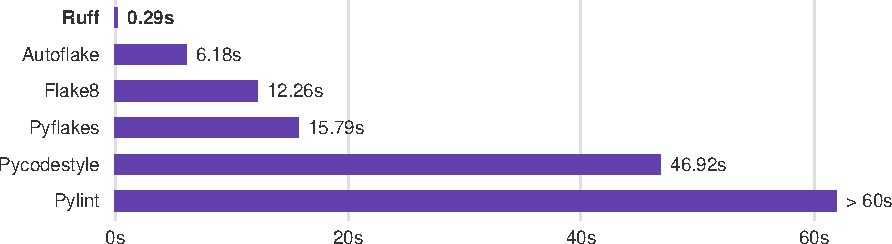
\includegraphics[width=0.7\textwidth]{graphics/speed_ruff.pdf}\src{docs.astral.sh/ruff}
  \end{center}
\end{frame}

\begin{splitframe}[fragile]{Surface Quality: Ruff}{pyproject.toml}
  \begin{columns}[t,onlytextwidth]
    \begin{column}{0.58\textwidth}
      {
      \usemintedstyle{code-light}
      \begin{itemize}
        \setlength{\itemsep}{2.5em}
        \item Install via \texttt{uv} as global tool or add to your project:
          \begin{minted}{shell-session}
            $ uv tool install ruff@latest
            $ uv add --dev ruff
          \end{minted}
        \item Two tools in one: \emph{Formatter} and \emph{linter}
          \begin{minted}{shell-session}
            $ ruff check
            $ ruff format
          \end{minted}
        \item Ruff supports over \emph{800} lint rules, inspired by the popular tools
          shown earlier \to{} See \iref{https://docs.astral.sh/ruff/rules/}{Rules}.
          \begin{itemize}
            \setlength{\itemsep}{1em}
            \item [\to] Configure everything in \texttt{pyproject.toml} or \texttt{ruff.toml}.
            \item [\to] Disable specific rules that you don't need in your project, \eg, \texttt{B905} \textit{zip-without-explicit-strict}.
          \end{itemize}
      \end{itemize}
      }
    \end{column}
    \hfill
    \begin{column}{0.38\textwidth}
      \footnotesize
      \vspace*{0.25cm}
      \begin{minted}{toml}
        [tool.ruff]
        target-version = "py313"
        line-length = 88
        extend-exclude = ["tests"]

        [tool.ruff.lint]
        extend-select = [
          "I",   # isort
          "E",   # pycodestyle
          "F",   # Pyflakes
          "UP",  # pyupgrade
          "B",   # flake8-bugbear
          "SIM", # flake8-simplify
        ]
        ignore = ["B905"]

        fixable = ["ALL"]
        unfixable = []

        [tool.ruff.lint.per-file-ignores]
        "examples/**" = ["I"]

        [tool.ruff.format]
        quote-style = "double"
        indent-style = "space"
        line-ending = "auto"
        skip-magic-trailing-comma = false
        docstring-code-format = true

        [tool.ruff.lint.isort]
        known-first-party = ["my_package"]
      \end{minted}
    \end{column}
  \end{columns}
\end{splitframe}

\begin{splitframe}[fragile]{Semantic Quality: Docstrings}{NumPy Style}
  \begin{columns}[t,onlytextwidth]
    \begin{column}{0.58\textwidth}
      {
      \usemintedstyle{code-light}
      \begin{itemize}
        \setlength{\itemsep}{2.5em}
        \item Explains what your code does.
        \item Can be understood by IDEs and autocompletion tools
        \item Necessary for well-written docs (later)
        \item Structure:
          \begin{itemize}
            \item [\to] Triple double quotes (\mintinline{python}+"""..."""+)
            \item Human-readable, complete sentences describing your code
            \item Explanation of parameters, returns, and exceptions
          \end{itemize}
        \item Many different styles available: Use \emph{one} and \emph{stick to it}.
      \end{itemize}
      }
    \end{column}
    \hfill
    \begin{column}{0.38\textwidth}
      \footnotesize
      \vspace*{0.25cm}
      \begin{minted}{python}
        def draw_sampling_opts(size: int) -> Dict:
            """Draws randomized sampling parameters
            for the simulation.

            Parameters
            ----------
            size : int
                Number of parameters to draw, equal
                to number of images.

            Returns
            -------
            samp_opts : dict
                Sampling options/parameters stored
                inside a dictionary.
            """
      \end{minted}
    \end{column}
  \end{columns}
\end{splitframe}

{
\usemintedstyle{code-light}
\begin{frame}[fragile]{Semantic Quality: Type Hinting}
  \begin{center}
    \huge\textcolor{ccyan}{Python is dynamically typed, but\dots}
  \end{center}
  \begin{itemize}
    \setlength{\itemsep}{1em}
    \item \dots you can still declare types for variables:
      \begin{minted}{python}
        foo: int = 1
        bar: str = "app"
        baz: np.ndarray = np.array([...])

        def func(a: int, b: int=42) -> int:
          return a + b
      \end{minted}
    \item [\to] Improved code readability
    \item IDE and linting support, \eg, through code completion
    \item But: Type hinting is \emph{not} enforced at runtime and one has
      to consider dynamic types

    \item Tools:
      \begin{description}[\iref{https://microsoft.github.io/pyright/}{pyright}]
        \item [\iref{https://mypy-lang.org/}{mypy}] Good for CI/CLI
        \item [\iref{https://microsoft.github.io/pyright/}{pyright}] Proprietary tool, but faster and with VSCode integration
      \end{description}
  \end{itemize}
\end{frame}
}

\begin{splitframe}[fragile]{Automation: pre-commit Hook}{.pre-commit-config.yaml}{0.5}
  \begin{columns}[t,onlytextwidth]
    \begin{column}{0.48\textwidth}
      {
      \usemintedstyle{code-light}
      \begin{itemize}
        \setlength{\itemsep}{2em}
        \item \iref{https://pre-commit.com/}{pre-commit} does all the formatting and linting for you
        \item Install via \texttt{uv}:
          \begin{minted}{shell-session}
            $ uv pip install pre-commit
          \end{minted}
        \item Many different hooks available:
          \begin{itemize}
            \item \texttt{ruff}, \texttt{mypy}, \iref{https://github.com/codespell-project/codespell}{codespell}, and many more\dots
          \end{itemize}
        \item Runs all tools defined in \texttt{.pre-commit-config.yaml}
        \item Run \mintinline{shell-session}+$ pre-commit install+ to install
          hooks in your project
        \item \mintinline{shell-session}{pre-commit} runs automatically whenever something is comitted
          using \mintinline{shell-session}{$ git commit ...}
      \end{itemize}
      }
    \end{column}
    \hfill
    \begin{column}{0.48\textwidth}
      \footnotesize
      \vspace*{0.25cm}
      \begin{minted}{yaml}
        repos:
          - repo: https://github.com/pre-commit/pre-commit-hooks
            rev: "v5.0.0"  # <- git version tag
            hooks:
              - id: check-added-large-files
              - id: check-case-conflict
              - id: check-merge-conflict
              - id: check-symlinks
              - id: check-yaml
              - id: debug-statements
              - id: end-of-file-fixer
              - id: mixed-line-ending
              - id: name-tests-test
                args: ["--pytest-test-first"]
              - id: requirements-txt-fixer
              - id: trailing-whitespace

          - repo: https://github.com/astral-sh/ruff-pre-commit
            rev: "v0.12.3"
            hooks:
              - id: ruff-format
              - id: ruff-check
                args: ["--fix", "--show-fixes"]

          - repo: https://github.com/codespell-project/codespell
            rev: v2.4.1
            hooks:
            - id: codespell
              additional_dependencies:
                - tomli
      \end{minted}
    \end{column}
  \end{columns}
\end{splitframe}

\begin{frame}{Further Reading: Code Quality}
  \begin{columns}[t,onlytextwidth]
    \begin{column}{0.48\textwidth}
      \begin{itemize}
        \setlength{\itemsep}{1em}
        \item \iref{https://indico.desy.de/event/43817/sessions/19711/attachments/97900/134904/Code\%20Quality\%20PYOPP.pdf}{Stefans Talk On Code Quality}
        \item \iref{https://peps.python.org/pep-0008/}{PEP8 – Style Guide for Python Code}
        \item \iref{https://docs.astral.sh/ruff/}{Ruff Docs}
        \item \iref{https://mypy.readthedocs.io/en/stable/}{mypy Docs}
        \item \iref{https://microsoft.github.io/pyright/}{pyright Docs}
        \item \iref{https://pre-commit.com/}{pre-commit}
        \item \iref{https://github.com/pre-commit/pre-commit-hooks}{pre-commit-hooks}
        \item \iref{https://github.com/codespell-project/codespell}{codespell}
      \end{itemize}
    \end{column}
    \begin{column}{0.48\textwidth}
      \begin{itemize}
        \item \iref{https://peps.python.org/pep-0484/}{PEP484 – Type Hints}
        \item \iref{https://peps.python.org/pep-0544/}{PEP 544 – Protocols: Structural subtyping}
        \item \iref{https://learn.scientific-python.org/development/guides/style/\#type-checking}{Scientific Python Library Development Guide: Type Checking}
        \item \iref{https://numpydoc.readthedocs.io/en/latest/format.html}{NumPy Style Guide}
        \item \iref{https://google.github.io/styleguide/pyguide.html}{Google Python Style Guide}
      \end{itemize}
    \end{column}
  \end{columns}
  \end{frame}

\secslide{Testing}

\begin{frame}{When Do We Need Tests?}
  \begin{center}
    \huge\textcolor{ccyan!90!cblack}{Imagine the following\dots}
  \end{center}
  \begin{itemize}
    \item You have written a package with a lot of code, \eg, multiple scripts
    \item You found a bug somewhere in your code
    \item You have not thought of possible edge cases during development
  \end{itemize}
  \vspace{1em}
  \begin{center}
    \huge\textcolor{cpink!90!cblack}{\to{} You will need to investigate your codebase for
    causes of the bug and even then the same bug may appear some time later}
  \end{center}
\end{frame}

\begin{frame}{Solution}
  \begin{center}
    \huge\textcolor{ccyan!90!cblack}{Write persistent tests \textbf{during development!}}\\
    \uncover<2>{\huge\textcolor{ccyan!90!cblack}{(And \textbf{automate} them \to{} see CI)}}

    \begin{tikzpicture}[remember picture, overlay]
      \only<2>{
        \node [anchor=south] at ([yshift=1cm]current page.south) {
          
\includegraphics[height=3cm]{graphics/automation_meme.png}
        };
      }
    \end{tikzpicture}
  \end{center}
\end{frame}

\begin{frame}{Test Levels}
  \begin{description}[Operational Acceptance Testing]
    \setlength{\itemsep}{1em}
    \item [Unit Testing] Test single units (\ie, single functions or classes) of your software.
    \item [Integration Testing] Test multiple components that depend on each other.
    \item [System Testing] Test the entire software with respect to its requirements, \eg, I/O data.
    \item [Operational Acceptance Testing] Give your software to the user to break it.
  \end{description}
  \vspace{0.5cm}
  \uncover<2>{
    \begin{center}
      
\includegraphics[height=3cm]{graphics/onedoesnot.jpg}
    \end{center}
  }
\end{frame}

\begin{frame}{What Do We Test For?}
  \begin{center}
    \huge\textcolor{ccyan}{This is probably the hardest part\dots}
  \end{center}
  \begin{itemize}
    \setlength{\itemsep}{1em}
    \item You will need to understand your code
    \item You will need to verify how much and what parts of your code are covered by tests
    \item Even then your code may not be guaranteed to work error-free
    \item \emph{Good practice}: Every time you find a bug, add a unit test so it doesn't reappear
  \end{itemize}
\end{frame}

{
  \usemintedstyle{code-light}
\begin{frame}[fragile]{Tools}
  Shipped with Python:
  \begin{description}
    \item [\iref{https://docs.python.org/3/library/doctest.html}{doctest}] Allows you to write simple tests in the docstrings
      of your functions.
    \item [\iref{https://docs.python.org/3/library/unittest.html}{unittest}] Allows you to write regular unit tests,
      \ie, separate functions and classes that test your code.
  \end{description}
  \vspace{0.5cm}

  Additional tools:
  \begin{description}[\iref{https://coverage.readthedocs.io/en/7.9.2/}{Coverage.py}]
    \item [\iref{https://docs.pytest.org/en/stable/}{pytest}] Scalable, extensible (\ie, through plugins), and easy to use test framework.
    \item [\iref{https://coverage.readthedocs.io/en/7.9.2/}{Coverage.py}] A tool for measuring code coverage. Works well with \texttt{pytest}
      if \iref{https://pytest-cov.readthedocs.io/en/latest/}{pytest-cov} is installed:
      \begin{minted}{shell-session}
        $ pytest --cov
      \end{minted}
    \item [\iref{https://tox.wiki/en/4.28.1/}{tox}] A generic virtual environment management and test command line tool. Can be used to:
      \begin{itemize}
        \item [\to] Check whether your package builds and installs in different envs
        \item [\to] Run tests in each defined env, \eg, using \texttt{pytest}
      \end{itemize}
    \item [\iref{https://nox.thea.codes/en/stable/}{Nox}] Similar to \texttt{tox}, but uses standard Python files and decorators for configuration.
      (For differences, see \iref{https://hynek.me/articles/why-i-like-nox/}{Why I Like Nox} by Hynek Schlawack)
  \end{description}
\end{frame}
}

\begin{darkframe}[fragile]{pytest}
  \begin{center}
    \large\textcolor{ccyan}{An example taken from the \texttt{pytest} docs}
  \end{center}
  \vspace{0.25cm}
  \begin{columns}[t,onlytextwidth]
    \begin{column}{0.28\textwidth}
      \begin{minted}{python}
        # test_sample.py
        def inc(x):
            return x + 1


        def test_answer():
            assert inc(3) == 5
      \end{minted}
    \end{column}
    \hfill
    \begin{column}{0.68\textwidth}
      \footnotesize
      % oh boi, the following caused me pain
      \begin{minted}[escapeinside=||]{shell-session}
        $ pytest test_sample.py
        =========================== test session starts ============================
        platform linux -- Python 3.x.y, pytest-8.x.y, pluggy-1.x.y
        rootdir: /home/sweet/project
        collected 1 item

        test_sample.py |\textcolor{cred}{F}|                                                     |\textcolor{cred}{[100\%]}|

        ================================= FAILURES =================================
        |\textcolor{cred}{\_\_\_\_\_\_\_\_\_\_\_\_\_\_\_\_\_\_\_\_\_\_\_\_\_\_\_\_\_\_\_ test\_answer \_\_\_\_\_\_\_\_\_\_\_\_\_\_\_\_\_\_\_\_\_\_\_\_\_\_\_\_\_\_\_\_}|

            def test_answer():
        >       assert inc(3) == 5
        |\textcolor{cred}{E}|       |\textcolor{cred}{assert 4 == 5}|
        |\textcolor{cred}{E}|        |\textcolor{cred}{+  where 4 = inc(3)}|

        |\textcolor{cred}{test\_sample.py}|:6: AssertionError
        |\textcolor{ccyan}{========================= short test summary info ==========================}|
        |\textcolor{cred}{FAILED}| test_sample.py::test_answer - assert 4 == 5
        |\textcolor{cred}{============================ 1 failed in 0.12s =============================}|
      \end{minted}
    \end{column}
  \end{columns}
\end{darkframe}

\begin{splitframe}[fragile]{pytest}{pyproject.toml}
  \begin{columns}[t,onlytextwidth]
    \begin{column}{0.58\textwidth}
      \begin{itemize}
        \setlength{\itemsep}{1em}
        \item \texttt{pytest} runs all functions starting with \texttt{test\_} (or classes starting with \texttt{Test}).
        \item Provide \texttt{pytest} with the file that contains the specific test functions you want to run.
        \item If no arguments are provided to \texttt{pytest}, it looks for paths defined in \texttt{testpath} (if defined)
          \begin{itemize}
            \item [\to] Otherwise: Recursive search for files matching \texttt{test\_*.py} or \texttt{*\_test.py}
          \end{itemize}
        \item Prints are suppressed per default; use the \texttt{-s} flag to see prints:
          {
          \usemintedstyle{code-light}
          \begin{minted}{shell-session}
            $ pytest -s
          \end{minted}
          }
      \end{itemize}
    \end{column}
    \begin{column}{0.38\textwidth}
      \begin{minted}{toml}
        [tool.pytest.ini_options]
        testpaths = [
          "tests",
        ]
        addopts = "--verbose"
      \end{minted}
    \end{column}
  \end{columns}
\end{splitframe}

\begin{darkframe}[fragile]{Useful Feature: pytest Fixtures}
  \begin{columns}[t,onlytextwidth]
    \begin{column}{0.38\textwidth}
      \small
      \begin{minted}{python}
        # contents of test_append.py (pytest)
        import pytest


        # Arrange
        @pytest.fixture
        def first_entry():
            return "a"


        # Arrange
        @pytest.fixture
        def order(first_entry):
            return [first_entry]


        def test_string(order):
            # Act
            order.append("b")

            # Assert
            assert order == ["a", "b"]
      \end{minted}
    \end{column}
    \begin{column}{0.58\textwidth}
      \small
      \begin{minted}{python}
        # radionets tests/conftest.py
        import shutil

        import pytest


        @pytest.fixture(autouse=True, scope="session")
        def test_suite_cleanup_thing():
            yield

            build = "./tests/build/"
            print("Cleaning up tests.")

            shutil.rmtree(build)
      \end{minted}
      \vspace{0.5cm}
      \normalsize
      \begin{itemize}
        \item [\to] \texttt{pytest} fixtures provide defined, reliable and consistent context for the tests
        \item [\to] Essentially code to be run before or after a test, \eg, to prepare objects, data, or files
      \end{itemize}
    \end{column}
  \end{columns}
\end{darkframe}

\begin{frame}{Testing: Good Practices}
  \textcolor{ccyan}{\textbf{Test-driven development:}}
  \begin{itemize}
      \item [\to] Make testing part of your development process
      \item [\to] Write tests \emph{before} implementing your code:
      \begin{enumerate}
        \item Specify what the code should do
        \item Write tests that test those specifications
        \item Implement the code
      \end{enumerate}
  \end{itemize}
  \vspace{1em}
  In reality this may not always be feasible, but\dots
  \begin{itemize}
    \item Always try to write tests for your code, especially for critical components
    \item You can always add tests at a later time, in a separate commit
    \item Always write tests when you found and fixed a bug to ensure it doesn't reappear
  \end{itemize}
\end{frame}

\begin{frame}{Further Reading: Testing}
  \begin{columns}[t,onlytextwidth]
    \begin{column}{0.48\textwidth}
        \begin{itemize}
          \setlength{\itemsep}{1em}
          \item \iref{https://indico.desy.de/event/43817/sessions/19708/attachments/97952/134999/nikolai_testing_pyopp_aachen_25.06.2025.pdf}{Nikolai Krug's PYOPP Talk}
          \item \iref{https://github.com/nikoladze/pyopp-pytest-tutorial}{Nikolai Krug's pytest Tutorial}
          \item \iref{https://docs.python.org/3/library/doctest.html}{doctest}
          \item \iref{https://docs.python.org/3/library/unittest.html}{unittest}
          \item \iref{https://docs.pytest.org/en/stable/}{pytest}
          \item \iref{https://coverage.readthedocs.io/en/7.9.2/}{Coverage.py}
          \item \iref{https://tox.wiki/en/4.28.1/}{tox}
        \end{itemize}
    \end{column}
    \begin{column}{0.48\textwidth}
      \begin{itemize}
        \setlength{\itemsep}{1em}
        \item \iref{https://nox.thea.codes/en/stable/}{Nox} and \iref{https://hynek.me/articles/why-i-like-nox/}{Why I Like Nox}
        \item \iref{https://pytest-xdist.readthedocs.io/}{pytest-xdist}
        \item \iref{https://pytest-regressions.readthedocs.io/}{pytest-regression}
        \item \iref{https://pytest-mock.readthedocs.io/}{pytest-mock}
        \item \iref{https://hypothesis.readthedocs.io/}{pytest-hypothesis}
        \item \iref{https://pytest-order.readthedocs.io/en/latest/}{pytest-order}
        \item \iref{https://henryiii.github.io/se-for-sci/content/week03/testing.html}{Intro To Testing} by Henry Schreiner
      \end{itemize}
    \end{column}
  \end{columns}
\end{frame}

\secslide{Documentation}

\begin{frame}{Why Should We Document Our Code?}
  \begin{center}
    \huge\textcolor{ccyan!90!cblack}{Well documented code improves\dots}
  \end{center}
  \begin{itemize}
    \item Maintainability: Future developers, debugging, \dots
    \item Accessibility: Make your package easier to understand for new users
    \item Collaboration: Docs as a shared knowledge source
  \end{itemize}
\end{frame}

\begin{frame}[fragile]{Tool Of Choice: Sphinx}
  \begin{columns}[t, onlytextwidth]
    \begin{column}{0.68\textwidth}
      \begin{itemize}
        \setlength{\itemsep}{1em}
        \item FOSS, extensible documentation generator written in Python
        \item Multiple output formats: \texttt{HTML}, \LaTeX, ePub, and more\dots
        \item Content is written using a mark-up language (\texttt{reST} or \texttt{MyST})
        \item Support for various docstring formats (some through extensions)
        \item Install via uv or mamba:
          \begin{minted}{text}
            $ uv pip install sphinx
            $ mamba install sphinx
          \end{minted}
      \end{itemize}
    \end{column}
    \hfill
    \begin{column}{0.38\textwidth}
      \begin{center}
      
\includegraphics[width=0.8\textwidth]{logos/sphinx-logo.pdf}
      \end{center}
    \end{column}
  \end{columns}
\end{frame}


{
\usemintedstyle{code-light}
\begin{frame}[fragile]{Getting Started}
  \begin{minted}[escapeinside=||]{shell-session}
    $ sphinx-quickstart docs
    |\textcolor{ccyan}{> Separate source and build directories (y/n) [n]:}| y
    |\textcolor{ccyan}{> Project name:}| ...
    |\textcolor{ccyan}{> Author name(s):}| ...
    |\textcolor{ccyan}{> Project release []:}| ...
    |\textcolor{ccyan}{> Project language [en]:}| ...
  \end{minted}

  \begin{center}
  \pause
  \begin{minipage}{.45\textwidth}
  \adjustbox{max height=5.5cm}{%
    \begin{forest}
      for tree={dir tree}
      [docs, opened
        [build, closed]
        [source, opened
          [\_static, closed]
          [\_templates, closed]
          [conf.py, pythonfile]
          [index.rst, textfile]
        ]
        [make.bat, batchfile]
        [Makefile, makefile]
      ]
    \end{forest}
  }
  \end{minipage}
  \hfill
  \pause
  \begin{minipage}{.45\textwidth}
    \adjustbox{max height=5.5cm}{%
      \begin{forest}
        for tree={dir tree}
        [docs, opened
          [\_build, closed]
          [\_static, closed]
          [\_templates, closed]
          [conf.py, pythonfile]
          [index.rst, textfile]
          [make.bat, batchfile]
          [Makefile, makefile]
        ]
      \end{forest}
    }
  \end{minipage}
  \end{center}
\end{frame}
}

{
\setbeamercolor{description item}{fg=cblack}
\begin{frame}[fragile]{Breakdown of the Generated Structure}
  \begin{description}[labelwidth=\widthof{\faFolderOpen \texttt{\_templates}}]
    \setlength{\itemindent}{-4em}
    \item [\textcolor{dircolor}{\faFolderOpen} \texttt{build}:] Output directory for the docs.
    \item [\textcolor{dircolor}{\faFolderOpen} \texttt{\_static}:] Directory for static elements such as images, icons, or logos.
    \item [\textcolor{dircolor}{\faFolderOpen} \texttt{\_templates}:] Used to store \iref{https://jinja.palletsprojects.com/en/stable/}{\texttt{Jinja}}
      templates for HTML page generation. %Also used by some Sphinx extensions.
    \item [\faFile* \texttt{index.rst}:] Root document; contains the root of the table of contents tree.
      % Effectively your landing page in the HTML version.
    \item [\faPython \texttt{conf.py}:] Main configuration file written in Python.
  \end{description}
\end{frame}
}

{
\usemintedstyle{code-light}
\begin{frame}[fragile]{Let's Build Our Docs}
  We will use the \texttt{Makefile} generated by \mintinline{shell-session}+sphinx-quickstart+ to build any format:
  \begin{minted}{shell-session}
    $ make <format>
  \end{minted}
  So, for the HTML version:
  \begin{minted}{shell-session}
    $ make html
  \end{minted}
  This will generate the HTML files for our docs inside the \texttt{build} directory.
  We can view the docs locally by running a Python HTTP server (in this case from inside the \texttt{docs} directory):
  \begin{minted}{shell-session}
    $ python -m http.server -d build/html [port]
  \end{minted}

  \begin{block}{Note}
    \mintinline{shell-session}+[port]+ is optional, see \mintinline{shell-session}+python -m http.server --help+.
  \end{block}
\end{frame}
}

\begin{darkframe}[fragile]{Setting Up conf.py}
  The \texttt{conf.py} file generated by Sphinx should look something like this:
  \begin{minted}{python}
    # -- Project information ------------------------
    project = 'pyopp'
    copyright = '2025, Author'
    author = 'Author'
    release = 'v0.1'

    # -- General configuration ----------------------
    extensions = []

    templates_path = ['_templates']
    exclude_patterns = []

    # -- Options for HTML output --------------------
    html_theme = 'alabaster'
    html_static_path = ['_static']
  \end{minted}
\end{darkframe}


\begin{darkframe}[fragile]{Setting Up conf.py | Project Information}
  \vspace*{0.25cm}
  Let's get some metadata from \texttt{pyproject.toml} using \texttt{tomli} or \texttt{tomllib} (Python $\geqslant$ \texttt{3.11}):\\[0.25\baselineskip]
  \footnotesize
  \begin{minted}{python}
    #!/usr/bin/env python3
    import datetime
    import sys
    from pathlib import Path

    import package                                                           # your package

    if sys.version_info < (3, 11):
        import tomli as tomllib
    else:
        import tomllib

    pyproject_path = Path(__file__).parent.parent.parent / "pyproject.toml"  # Get path of pyproject.toml
    pyproject = tomllib.loads(pyproject_path.read_text())                    # Load contents

    project = pyproject["project"]["name"]                                   # Get project name
    author = pyproject["project"]["authors"][0]["name"]                      # Get author name
    copyright = "{}.  Last updated {}".format(
        author, datetime.datetime.now().strftime("%d %b %Y %H:%M")
    )                                                                        # Set copyright string
    python_requires = pyproject["project"]["requires-python"]                # Get minimum python version requirement
    rst_epilog = f"""
    .. |python_requires| replace:: {python_requires}
    """                                                                      # Make python_requires var accessible

    version = package.__version__                                            # Get version
    release = version                                                        # Full release version
  \end{minted}
\end{darkframe}


\begin{darkframe}[fragile]{Setting Up conf.py | General Configuration}
  Sphinx extensions add functionality and customization. The following extensions
  are some of the extensions we always use in our docs:\\[0.25\baselineskip]
    \small
    \begin{minted}{python}
      extensions = [
          "sphinx.ext.autodoc",                # Imports modules and pulls in documentation from docstrings
          "sphinx.ext.intersphinx",            # Cross-references to other projects
          "sphinx.ext.coverage",               # Collects doc coverage stats
          "sphinx.ext.viewcode",               # Links to highlighted source code (i.e. "[source]" button)
          "sphinx_automodapi.automodapi",                    # Automatically generates module documentation
          "sphinx_automodapi.smart_resolver",                # Helps resolving some imports
          "numpydoc",                                        # Support for the NumPy docstring format
          "IPython.sphinxext.ipython_console_highlighting",  # Syntax highlighting of ipython prompts
          "sphinx_copybutton",                               # Adds a copybutton to code blocks
      ]
    \end{minted}
\end{darkframe}

{
\usemintedstyle{code-light}
\begin{frame}[fragile]{Setting Up \texttt{conf.py} | General Configuration}
    Some extensions are not shipped with Sphinx and need to be installed separately in your environment:
    \begin{minted}{shell-session}
      $ mamba install sphinx-automodapi numpydoc pydata-sphinx-theme sphinx-copybutton
    \end{minted}
    or with \texttt{uv}
    \begin{minted}{shell-session}
      $ uv pip install sphinx-automodapi numpydoc pydata-sphinx-theme sphinx-copybutton
    \end{minted}
\end{frame}
}

\begin{darkframe}[fragile]{Setting Up conf.py | General Configuration}
  Now we can set up some more settings for the extensions:\\[0.25\baselineskip]
    \begin{minted}{python}
    # gets rid of some errors during build
    numpydoc_show_class_members = False
    numpydoc_class_members_toctree = False

    intersphinx_mapping = {
       "numpy": ("https://numpy.org/doc/stable", None),
       ...
    }

    suppress_warnings = ["intersphinx.external"]  # sometimes necessary

    templates_path = ["_templates"]
    exclude_patterns = ["build", "Thumbs.db", ".DS_Store", "changes", "*.log"]

    source_suffix = {".rst": "restructuredtext"}  # Set .rst files as source files for docs
    master_doc = "index"                          # index.rst as root file
  \end{minted}
\end{darkframe}

\begin{darkframe}[fragile]{Setting Up conf.py | HTML And Theme Options}
  HTML options set the look of your docs. The Sphinx community has created a variety of
  themes you can choose from.\\[0.25\baselineskip]
  \begin{minted}{python}
    html_theme = "pydata_sphinx_theme"            # Modern, widely used theme

    html_static_path = ["_static"]
    html_favicon = "_static/favicon/favicon.ico"  # Icon file for browser tabs
    html_css_files = ["custom.css"]               # Custom CSS settings like colors or fonts
    html_file_suffix = ".html"

    html_theme_options = {...}                    # Depends on the theme

    html_title = f"{project}"                     # e.g. your project name
    htmlhelp_basename = project + " docs"
  \end{minted}
  \vspace{0.25\baselineskip}
  Check out \emph{Sphinx Themes Gallery} for a curated list of available themes:
  \iref{https://sphinx-themes.org/}{sphinx-themes.org}
\end{darkframe}


\begin{darkframe}[fragile]{Filling the Docs: Landing Page}
    \footnotesize
    \begin{minted}{rst}
      :html_theme.sidebar_secondary.remove: true
      :html_theme.sidebar_primary.remove: true

      .. _package:

      =======
      Package
      =======

      .. currentmodule:: package

      **Version**: |version| | **Date**: |today|

      **Useful links**: `Source Repository <https://github.com/your_project/package>`__ |
      `Issue Tracker <https://github.com/your_project/package/issues>`__ |
      `Pull Requests <https://github.com/your_project/package/pulls>`__

      **License**: `MIT <https://github.com/your_project/package/blob/main/LICENSE>`__

      **Python**: |python_requires|

      .. toctree::
         :maxdepth: 1
         :hidden:

         api-reference/index
         changelog
    \end{minted}
\end{darkframe}


\begin{frame}[fragile]{Filling the Docs: API References}
  We will create the API references (semi-)automatically in a few steps:
  \begin{columns}[onlytextwidth]
    \begin{column}{0.48\textwidth}
      \begin{enumerate}
        \item <1-> Copy the structure of your actual package
        \item <2-> Populate every subdirectory with a \texttt{index.rst}
        \item <3-> Create separate \texttt{.rst} files for every submodule
      \end{enumerate}
      \vspace{0.25cm}
      \begin{center}
        \adjustbox{max height=5cm}{%
          \begin{forest}
            for tree={dir tree}
            [package, opened
              [module1, opened
                [\_\_init\_\_.py, pythonfile]
                [submodule\_a.py, pythonfile]
                [submodule\_b.py, pythonfile]
              ]
              [module2, opened
                [\_\_init\_\_.py, pythonfile]
                [submodule\_c.py, pythonfile]
              ]
              [\_\_init\_\_.py, pythonfile]
            ]
          \end{forest}
        }
      \end{center}
    \end{column}
    \begin{column}{0.48\textwidth}
      \begin{center}
        % \adjustbox{max height=5cm}{%
          \begin{forest}
            for tree={dir tree}
            [docs, opened
              [api-reference, opened
                [module1, opened
                  [index.rst, textfile, visible on=<2->]
                  [submodule\_a.rst, textfile, visible on=<3->]
                  [submodule\_b.rst, textfile, visible on=<3->]
                ]
                [module2, opened
                  [index.rst, textfile, visible on=<2->]
                  [submodule\_c.rst, textfile, visible on=<3->]
                ]
                [index.rst, textfile, visible on=<2->]
              ]
              [...]
            ]
          \end{forest}
        % }
      \end{center}
    \end{column}
  \end{columns}
\end{frame}


\begin{darkframe}[fragile]{Filling the Docs: API References}
  For now, the API reference will still be empty. We have to fill in
  the \texttt{index.rst} files to change that. Starting with
  \texttt{api-reference/index.rst}:\\[1em]

  \begin{columns}[onlytextwidth]
    \begin{column}{0.38\textwidth}
      \begin{minted}{rst}
        .. _api-reference:

        *************
        API Reference
        *************

        .. toctree::
          :maxdepth: 1
          :glob:

          */index
      \end{minted}
    \end{column}
    \hfill
    \begin{column}{0.58\textwidth}
      We add\dots
      \begin{enumerate}
        \setlength{\itemsep}{1.5em}
        \item A tag \texttt{.. \_api-reference:} to the file so we can reference it if necessary
        \item A title, \eg, \enquote{API Reference}
        \item The table of contents with the \texttt{.. toctree::} directive
          \begin{itemize}
            \item And add only \texttt{index.rst} files from the subdirectories to the TOC
          \end{itemize}
      \end{enumerate}
    \end{column}
  \end{columns}
\end{darkframe}

\begin{darkframe}[fragile]{Filling the Docs: API References}

  \begin{columns}[onlytextwidth]
    \begin{column}{0.52\textwidth}
      \scriptsize
      \begin{minted}{rst}
        .. _module1:

        ********************************
        Module1 (:mod:`package.module1`)
        ********************************

        .. currentmodule:: package.module1

        Introduction
        ============

        :mod:`package.module1` contains useful methods and classes.

        Submodules
        ==========

        .. toctree::
          :maxdepth: 1
          :glob:

          submodule_a
          submodule_b

        Reference/API
        =============

        .. automodapi:: package.module1
            :no-inheritance-diagram:
      \end{minted}
    \end{column}
    \hfill
    \begin{column}{0.46\textwidth}
      Now, we do the same for the \texttt{index.rst} files in the module directories:\\[1em]
      We add\dots
      \begin{enumerate}
        \setlength{\itemsep}{1.5em}
        \item A tag and module title
        \item The \texttt{.. currentmodule::} directive to let Sphinx know that
          classes and functions documented from here on are in the given module
        \item (optional) Some introduction to the module
        \item The table of contents for the submodules of the module
        \item The \texttt{.. automodapi::} directive for the current module to get a list of
          classes and functions
      \end{enumerate}
    \end{column}
  \end{columns}
\end{darkframe}

\begin{darkframe}[fragile]{Filling the Docs: API References}
  Finally, we write the submodule \texttt{.rst} files:

  \begin{columns}[onlytextwidth]
    \begin{column}{0.5\textwidth}
      \footnotesize
      \begin{minted}{rst}
        .. _data:

        ************************************************
        submodule_a (:mod:`package.module1.submodule_a`)
        ************************************************

        .. currentmodule:: package.module1.submodule_a

        Submodule of :mod:`package.module1`.


        Reference/API
        =============

        .. automodapi:: package.module1.submodule_a
            :inherited-members:
      \end{minted}
    \end{column}
    \hfill
    \begin{column}{0.46\textwidth}
      We add\dots
      \begin{enumerate}
        \setlength{\itemsep}{1.5em}
        \item A tag, the submodule title, and the\\\texttt{.. currentmodule::} directive
        \item (optional) Some introduction to the submodule
        \item The \texttt{.. automodapi::} directive for the current submodule to get a list of
          classes and functions
      \end{enumerate}
    \end{column}
  \end{columns}
\end{darkframe}

{
\usemintedstyle{code-light}
\begin{frame}[fragile]{reST: Headings}
  \begin{columns}[t, onlytextwidth]
    \begin{column}{0.33\textwidth}
        \begin{minted}{rst}
          ####
          Part
          ####

          *******
          Chapter
          *******

          Section
          =======

          Subsection
          ----------

          Subsubsection
          ^^^^^^^^^^^^^

          Paragraph
          """""""""
        \end{minted}
    \end{column}
    \hfill
    \begin{column}{0.66\textwidth}
      \begin{itemize}
        \setlength{\itemsep}{1.5em}
        \item The structure is technically determined by order of occurance
        \begin{itemize}
          \item \textbf{But}: For better readability stick to the same order throughout your docs, \eg, the one shown here (recommended)
        \end{itemize}
        \item While overlines are optional, they are encouraged for parts and chapters
        \item Any of the following symbols are valid for over- and underlines:\\
          \textcolor{cpink}{\texttt{\#} \texttt{*} \texttt{=} \texttt{-} \texttt{\textasciicircum} \texttt{"} \texttt{+} \texttt{\_} \texttt{\textasciitilde}}
          \mintinline{text}{` . , : ; ' ! ? & $ %}
          \mintinline{text}+( ) [ ] { }+\\
          \mintinline{text}+< > @ \ / |+
      \end{itemize}
    \end{column}
  \end{columns}
\end{frame}

\begin{frame}[fragile]{reST: Roles, Directives, and Field Lists}
  \begin{itemize}
    \setlength{\itemsep}{1em}
    \item Roles are \textbf{inline} pieces of explicit markup that are understood by Sphinx.
    The syntax is:
    \begin{center}
      \begin{minted}{rst}
        :rolename:`content`
      \end{minted}
    \end{center}

  \item [\to] Examples:
    \begin{minted}{rst}
      :mod:`package.module1` :code:`foo = 42` :math:`F = m\cdot a`
    \end{minted}

  \item Directives are \textbf{blocks} of explicit markup that are understood by Sphinx.
    The syntax is:
    \begin{center}
      \footnotesize
      \begin{minted}{rst}
        .. directive:: [(optional) arguments]
           [:(optional) field list:] [(optional) field list value]

           [Body elements of the directive]
      \end{minted}
    \end{center}

  \item [\to] Examples:
    \footnotesize
    \begin{minted}{rst}
      .. image:: picture.png
         :width: 90%
         :alt: A nice picture.

      .. code-block::
         :caption: A code block.

         def func(param: int) -> int: ...
    \end{minted}
  \end{itemize}
\end{frame}
}

\begin{frame}[fragile]{Hosting on \rtd}
  \begin{itemize}
    \setlength{\itemsep}{1.5em}
    \item Free, if your package is open-source, \ie, publically available on, \eg, GitHub or GitLab and
      no handling of secrets required
    \item Allows you to preview your docs on every PR
    \item Works seamlessly with Sphinx
    \item Automatically builds the docs from your \texttt{main} branch
    \item Supports downloading the docs in PDF or other formats
  \end{itemize}
\end{frame}

\begin{darkframe}[fragile]{Hosting on \rtd}
  \begin{enumerate}
    \item Set up a \texttt{.readthedocs.yaml} file in your repository:
        \begin{minted}{yaml}
          version: 2

          build:
            os: ubuntu-24.04
            apt_packages:
              - graphviz
            tools:
              python: "3.13"
            jobs:
              pre_create_environment:
                  - asdf plugin add uv
                  - asdf install uv latest
                  - asdf global uv latest
              install:
                - uv pip install --upgrade pip  # <- may be necessary if pip < 25
                - uv pip install --group docs .

          sphinx:
            configuration: docs/conf.py
        \end{minted}
  \end{enumerate}
\end{darkframe}

\begin{frame}[fragile]{Hosting on \rtd}
  \begin{columns}[onlytextwidth]
    \begin{column}{0.48\textwidth}
      \begin{enumerate}
        \setlength{\itemsep}{1em}
        \setcounter{enumi}{1}
      \item <1-> Sign up/log in to \iref*{https://about.readthedocs.com/}{\rtd{}} (Community), \eg, via GitHub, GitLab, or Bitbucket
        \item <2-> In your dashboard, click on \enquote{Add project}
        \item <3-> Search for your repository and click \enquote{Continue}
        \item <4-> Configure the basic settings and click \enquote{Next}
        \item <5-> Ensure the \texttt{.readthedocs.yaml} file exists in your repository, and click \enquote{This file exists}
        \item <6-> Your docs should now be building and will be rebuilt anytime a PR is merged into \texttt{main}
      \end{enumerate}
    \end{column}
    \hfill
    \begin{column}{0.48\textwidth}
      \only<2>{
        
\includegraphics[width=\textwidth]{graphics/rtd1.png}
      }
      \only<3>{
        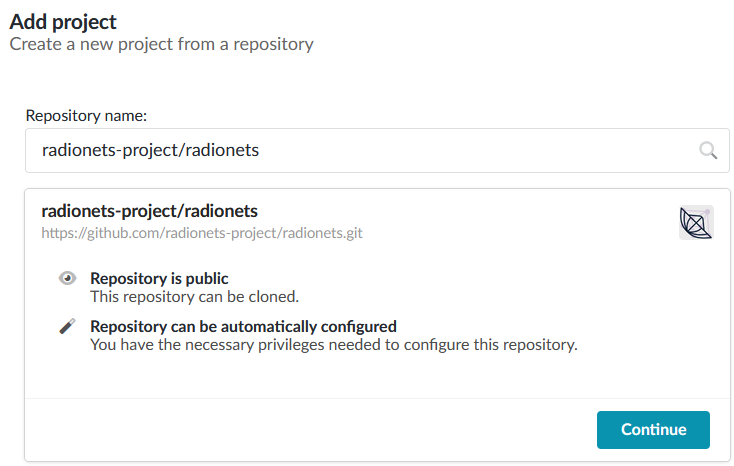
\includegraphics[width=\textwidth]{graphics/rtd2.png}
      }
      \only<4>{
        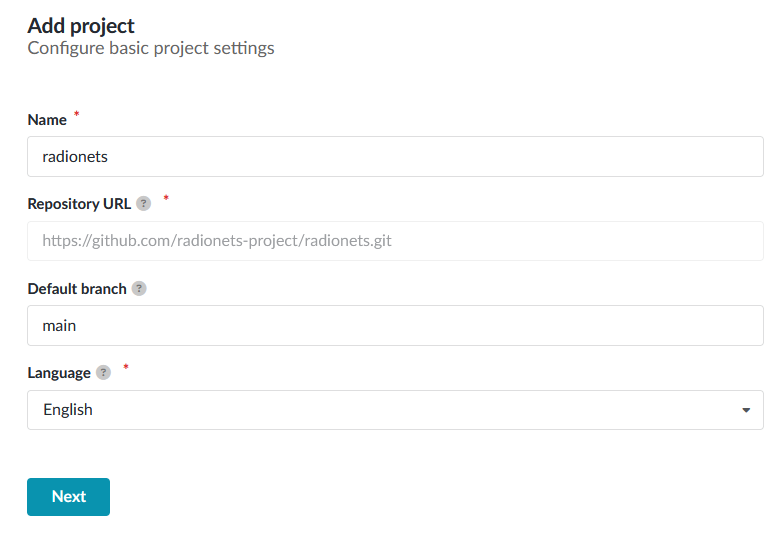
\includegraphics[width=\textwidth]{graphics/rtd3.png}
      }
      \only<5>{
        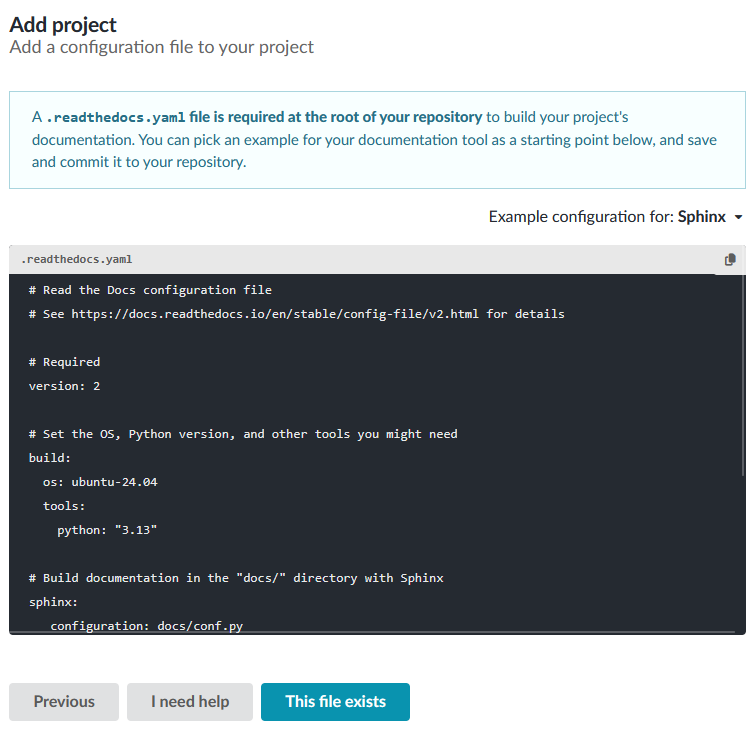
\includegraphics[width=\textwidth]{graphics/rtd4.png}
      }
      \only<6>{
        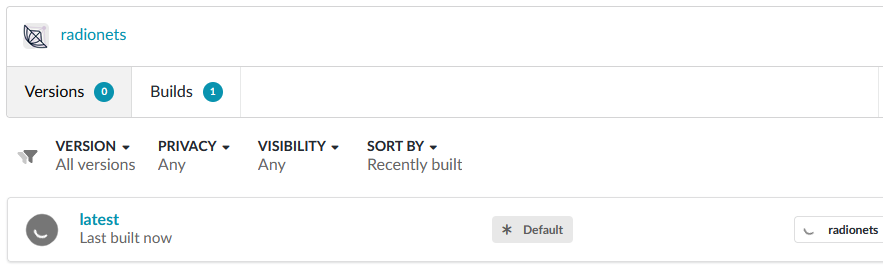
\includegraphics[width=\textwidth]{graphics/rtd5.png}
      }
    \end{column}
  \end{columns}
\end{frame}

\begin{frame}{Further Reading: Docs}
  \begin{columns}[t,onlytextwidth]
    \begin{column}{0.48\textwidth}
      \begin{itemize}
        \setlength{\itemsep}{1em}
        \item \iref{https://indico.desy.de/event/43817/sessions/19712/attachments/97983/135044/docs_ci_pyopp_2025.pdf}{My PYOPP Talk}
        \item \iref{https://www.sphinx-doc.org/en/master/}{Sphinx}
        \item \iref{https://github.com/sphinx-doc/sphinx-autobuild}{sphinx-autobuild}
        \item \iref{https://docs.python.org/3/reference/import.html}{Import System}
        \item \iref{https://peps.python.org/pep-0420/}{PEP 420 – Implicit Namespace Packages}
        \item \iref{https://www.sphinx-doc.org/en/master/usage/restructuredtext/basics.html}{reStructuredText (reST)}
        \item \iref{https://www.sphinx-doc.org/en/master/usage/restructuredtext/roles.html}{Roles}
        \item \iref{https://www.sphinx-doc.org/en/master/usage/restructuredtext/directives.html}{Directives}
      \end{itemize}
    \end{column}
    \begin{column}{0.48\textwidth}
      \begin{itemize}
        \setlength{\itemsep}{1em}
        \item \iref{https://www.sphinx-doc.org/en/master/usage/restructuredtext/field-lists.html}{Field Lists}
        \item \iref{https://towncrier.readthedocs.io/en/stable/index.html}{Towncrier} (Changelogs)
        \item \iref{https://sphinx-automodapi.readthedocs.io/en/latest/}{sphinx-automodapi}
        \item \iref{https://pydata-sphinx-theme.readthedocs.io/en/stable/}{PyData Sphinx Theme}
        \item \iref{https://numpydoc.readthedocs.io/en/latest/index.html}{numpydoc}
        \item \iref{https://sphinx-design.readthedocs.io/en/latest/}{sphinx-design}
        \item \iref{https://sphinx-gallery.github.io/stable/index.html}{sphinx-gallery}
      \end{itemize}
    \end{column}
  \end{columns}
\end{frame}

\secslide[\fontsize{1cm}{1cm}\selectfont]{Continuous Integration (CI),\\ Deployment,\\ and Continuous Delivery (CD)}

\begin{frame}[fragile]{What is Continuous Integration?}
  \begin{itemize}
    \setlength{\itemsep}{1em}
    \item A practice where tests and builds are run automatically, \eg, after code changes were
      merged/committed
    \item Goal: Find bugs, improve software quality (\eg, performance) and ensure
      your software runs on different platforms
    \item Every commit triggers a CI job
    \item Addressing failed CI jobs before merging a PR ensures code quality
    \item Running tests locally before committing adds an extra layer of ensuring code quality
  \end{itemize}
  \begin{block}{Note}
     The quality of your CI strongly depends on the quality of your tests.
     \begin{itemize}
      \item [\to] Requires effort beforehand.
     \end{itemize}
  \end{block}
\end{frame}


\begin{darkframe}[fragile]{CI: Multiple Platforms | GitHub Actions}
  \begin{enumerate}
        \begin{minted}{yaml}
          name: CI

          on:
            push:
              branches:
                - main
              tags:
                - '**'
            pull_request:

          env:
            MPLBACKEND: Agg
            PYTEST_ADDOPTS: --color=yes
        \end{minted}
  \end{enumerate}
\end{darkframe}

\begin{darkframe}[fragile]{CI: Multiple Platforms | GitHub Actions}
  \begin{enumerate}
    \setcounter{enumi}{1}
    \item We will be using GitHub Actions' matrix strategy to define multiple platforms:
        \scriptsize
        \begin{minted}{yaml}
          jobs:
            tests:
              runs-on: ${{ matrix.os }}
              strategy:
                matrix:
                  include:
                    - os: ubuntu-latest
                      python-version: "3.10"
                      install-method: mamba

                    - os: ubuntu-latest
                      python-version: "3.12"
                      install-method: mamba
                      extra-args: ["codecov"]  # lead platform for code cov

                    - os: ubuntu-latest
                      python-version: "3.12"
                      install-method: pip

                    - os: macos-13
                      python-version: "3.10"
                      install-method: pip

              defaults:
                run:
                  # We need login shells (-l) for micromamba to work.
                  shell: bash -leo pipefail {0}
        \end{minted}
  \end{enumerate}
\end{darkframe}

\begin{darkframe}[fragile]{CI: Multiple Platforms | GitHub Actions}
  \begin{enumerate}
    \setcounter{enumi}{2}
    \item Adding steps:
        \scriptsize
        \begin{minted}{yaml}
            steps:
              - uses: actions/checkout@v4
                with:
                  fetch-depth: 0

              - name: Prepare mamba installation
                if: matrix.install-method == 'mamba' &&  contains(github.event.pull_request.labels.*.name, 'documentation-only') == false
                env:
                  PYTHON_VERSION: ${{ matrix.python-version }}
                run: |
                  # setup correct python version
                  sed -i -e "s/- python=.*/- python=$PYTHON_VERSION/g" environment.yml

              - name: mamba setup
                if: matrix.install-method == 'mamba' && contains(github.event.pull_request.labels.*.name, 'documentation-only') == false
                uses: mamba-org/setup-micromamba@v1
                with:
                  environment-file: environment.yml
                  cache-downloads: true

              - name: Python setup
                if: matrix.install-method == 'pip' && contains(github.event.pull_request.labels.*.name, 'documentation-only') == false
                uses: actions/setup-python@v5
                with:
                  python-version: ${{ matrix.python-version }}
                  check-latest: true
        \end{minted}
  \end{enumerate}
\end{darkframe}

\begin{darkframe}[fragile]{CI: Multiple Platforms | GitHub Actions}
  \begin{enumerate}
    \setcounter{enumi}{3}
    \item For macOS, we have to fix the Python path:
        \scriptsize
        \begin{minted}{yaml}
          steps:
            - ...

            - if: matrix.install-method == 'pip' && runner.os == 'macOS' && contains(github.event.pull_request.labels.*.name, 'documentation-only') == false
              name: Fix Python PATH on macOS
              run: |
                tee -a ~/.bash_profile <<<'export PATH="$pythonLocation/bin:$PATH"'
        \end{minted}
  \end{enumerate}
\end{darkframe}

\begin{darkframe}[fragile]{
    Multiple Platforms | GitHub Actions
  }
  \begin{enumerate}
    \setcounter{enumi}{4}
    \item Install dependencies and run tests:
        \footnotesize
        \begin{minted}{yaml}
          steps:
            - ...

            - uses: astral-sh/setup-uv@v6

            - name: Install dependencies
              env:
                PYTHON_VERSION: ${{ matrix.python-version }}
              run: |
                python --version
                uv pip install --group tests -e .
                uv pip freeze
                uv pip list

            - name: List installed package versions (conda)
              if: matrix.environment-type == 'mamba'
              run: micromamba list

            - name: Tests
              run: |
                pytest -vv --cov --cov-report=xml

            - name: Upload coverage to Codecov
              uses: codecov/codecov-action@v4
              env:
                CODECOV_TOKEN: ${{ secrets.CODECOV_TOKEN }}  # make sure you have this set as repository secret
        \end{minted}
  \end{enumerate}
\end{darkframe}


\begin{darkframe}[fragile]{Codecov}
  \begin{enumerate}
    \item Sign up/log in to Codecov, \eg, via GitHub, GitLab, or Bitbucket
    \item Select your repository from your dashoard
    \item Select a setup option, \eg, \enquote{Using GitHub Actions}
    \item Select an upload token. For a single repository, the repository
      token is sufficient
    \item Add the token as repository secret
    \item Update your CI to automatically upload the coverage to Codecov (after the \texttt{Tests} step of your job)
      \begin{minted}{yaml}
        - name: Tests
          run: |
            pytest -vv --cov --cov-report=xml

        - name: Upload coverage to Codecov
          uses: codecov/codecov-action@v4
          env:
            CODECOV_TOKEN: ${{ secrets.CODECOV_TOKEN }}
      \end{minted}
  \end{enumerate}
  \vspace{0.25em}
  \begin{center}
    \huge\textcolor{cpink}{\to{} \textbf{NEVER} share your token with anyone.}
  \end{center}
\end{darkframe}


\begin{darkframe}[fragile]{Linting With the CI}
  \begin{center}
    
\includegraphics[height=3cm]{graphics/hank.jpg}\\[0.5\baselineskip]
    \huge\textcolor{ccyan}{%
      This is easier than ever: Set up your \texttt{.pre-commit-config.yaml},
      then go to \iref{pre-commit.ci/}{pre-commit.ci} and add your project/repository.
    }
  \end{center}
\end{darkframe}

\begin{darkframe}[fragile]{Building the Docs With the CI}
  The docs job can be started last.
  \footnotesize
    \begin{minted}{yaml}
      jobs:
        docs:
            runs-on: ubuntu-24.04
            steps:
              - uses: actions/checkout@v4
                with:
                  fetch-depth: 0

              - name: Set up Python
                uses: actions/setup-python@v5
                with:
                  python-version: "3.12"

              - name: Install doc dependencies
                run: |
                  sudo apt update -y && sudo apt install -y git build-essential pandoc graphviz ffmpeg
                  pip install -U pip towncrier setuptools
                  pip install -e .[docs]
                  git describe --tags

              - name: Build docs
                run: make -C docs html
    \end{minted}
\end{darkframe}

\begin{darkframe}{CI/CD: DevOps}
  \begin{center}
    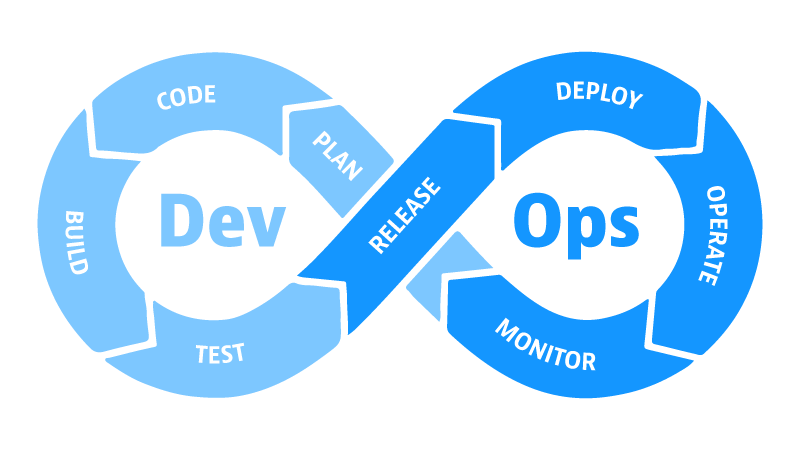
\includegraphics[height=0.6\textheight]{graphics/devops.png}
  \end{center}
\end{darkframe}

\begin{darkframe}[fragile]{CD: Publish on PyPI}
  \begin{minted}{yaml}
    name: Build Python Package

    on:
      push:
      workflow_dispatch:
      release:
        types:
          - published

    jobs:
      dist:
        runs-on: ubuntu-latest
        steps:
          - uses: actions/checkout@v4
          - uses: hynek/build-and-inspect-python-package@v2
            with:
              path: .
  \end{minted}
\end{darkframe}

\begin{darkframe}{CD: Publish on PyPI (cont.)}
  \begin{minted}{yaml}
    jobs:
      distlong:
        runs-on: ubuntu-latest
        steps:
          - uses: actions/checkout@v4
            with:
              fetch-depth: 0

          - uses: astral-sh/setup-uv@v6

          - name: Build SDist and wheel
            run: uvx --from build pyproject-build

          - uses: actions/upload-artifact@v4
            with:
              name: Packages-distlong-${{ github.job }}
              path: dist/*

          - name: Check metadata
            run: uvx twine check ./dist/*
  \end{minted}
\end{darkframe}

\begin{darkframe}{CD: Publish on PyPI (cont.)}
  \begin{minted}{yaml}
    jobs:
      publishtrusted:
        needs: [ dist ]
        environment: pypi
        permissions:
          id-token: write
          attestations: write
          contents: read
        runs-on: ubuntu-latest
        if: github.event_name == 'release' && github.event.action == 'published'
        steps:
          - uses: actions/download-artifact@v4
            with:
              name: Packages
              path: dist

          - name: Generate artifact attestation for sdist and wheel
            uses: actions/attest-build-provenance@v2
            with:
              subject-path: "./dist/*"

          - uses: pypa/gh-action-pypi-publish@release/v1
  \end{minted}
\end{darkframe}

\begin{frame}{Further Reading: CI/CD}
  \begin{columns}[t,onlytextwidth]
    \begin{column}{0.48\textwidth}
      \begin{itemize}
        \setlength{\itemsep}{1em}
        \item \iref{https://docs.google.com/presentation/d/1em_YjW-KcbQZLbNVL5izIJHiBxeMOq7GsSilcDoDIx0/}{Jonas Eschle's PYOPP Talk}
        \item \iref{https://indico.desy.de/event/43817/sessions/19712/attachments/97983/135044/docs_ci_pyopp_2025.pdf}{My PYOPP Talk}
        \item \iref{https://docs.github.com/en/actions}{GitHub Actions}
        \item \iref{https://github.com/actions/checkout}{actions/checkout}
        \item \iref{https://github.com/astral-sh/setup-uv}{astral-sh/setup-uv}
        \item \iref{https://github.com/mamba-org/setup-micromamba}{setup-micromamba}
      \end{itemize}
    \end{column}
    \begin{column}{0.48\textwidth}
      \begin{itemize}
        \setlength{\itemsep}{1em}
        \item \iref{https://docs.codecov.com/docs/}{Codecov}
        \item \iref{https://docs.github.com/en/actions/writing-workflows/choosing-what-your-workflow-does/running-variations-of-jobs-in-a-workflow}{Matrix Strategies}
        \item \iref{https://pre-commit.ci/}{pre-commit.ci}
        \item \iref{https://docs.gitlab.com/ci/}{GitLab CI}
        \item \iref{https://docs.gitlab.com/ci/variables/predefined_variables/}{GitLab: Predefined Variables}
        \item \iref{https://badge.fury.io/}{badge.fury.io} and \iref{https://shields.io/}{shields.io} (Badges)
      \end{itemize}
    \end{column}
  \end{columns}
\end{frame}


\begin{frame}
  \begin{center}
    
\includegraphics[height=0.75\textheight]{graphics/homer.jpg}
  \end{center}
\end{frame}

\end{document}
